\documentclass[xcolor=pdftex,dvipsnames,table,mathserif,aspectratio=169]{beamer}
\usetheme{metropolis}

%\usetheme{Darmstadt}
%\usepackage{times}
%\usefonttheme{structurebold}

\usepackage[english]{babel}
%\usepackage[table]{xcolor}
\usepackage{pgf,pgfarrows,pgfnodes,pgfautomata,pgfheaps}
\usepackage{amsmath,amssymb,setspace,centernot}
\usepackage[latin1]{inputenc}
\usepackage[T1]{fontenc}
\usepackage{relsize}
\usepackage{stmaryrd}
\usepackage{pdfpages}
\usepackage{booktabs}
\usepackage[absolute,overlay]{textpos} 


\newenvironment{reference}[2]{% 
  \begin{textblock*}{\textwidth}(#1,#2) 
      \footnotesize\it\bgroup\color{red!50!black}}{\egroup\end{textblock*}} 

\DeclareMathSizes{10}{10}{6}{6} 
\AtBeginSection[]{
  \begin{frame}
  \vfill
  \centering
  \begin{beamercolorbox}[sep=8pt,center,shadow=true,rounded=true]{title}
    \usebeamerfont{title}\insertsectionhead\par%
  \end{beamercolorbox}
  \vfill
  \end{frame}
}
\begin{document}
\title{Diversion Ratios}
\author{Chris Conlon}
\institute{Grad IO}
\date{\today}

\frame{\titlepage}
\section{What are Diversion Ratios?} 

\begin{frame}{Horizontal Merger Guidelines (2010 rev.)}
\begin{quote}
In some cases, the Agencies may seek to quantify the extent of direct competition between a product sold by one merging firm and a second product sold by the other merging firm by estimating the diversion ratio from the first product to the second product. The diversion ratio is the \alert{fraction of unit sales lost by the first product due to an increase in its price that would be diverted to the second product}. Diversion ratios between products sold by one merging firm and products sold by the other merging firm can be very informative for assessing unilateral price effects, with \alert{higher diversion ratios indicating a greater likelihood of such effects}. Diversion ratios between products sold by merging firms and those sold by \alert{non-merging firms have at most secondary predictive value.}
\end{quote}
\end{frame}

\begin{frame}{This time with equations}
 Raise price of good $j$. People leave. What fraction of leavers switch to $k$?
\begin{eqnarray*}
D_{jk} (p_j,p_{-j})= \frac{\frac{\partial q_k}{\partial p_j}}{\left|\frac{\partial q_j}{\partial p_j} \right|}
\end{eqnarray*}
It's one of the best ways economists have to characterize competition among sellers.
\begin{itemize}
\item High Diversion: Close Substitutes $\rightarrow$ Mergers more likely to increase prices.
\item Very low diversion $\rightarrow$ products may not be in the same market.\\ (ie: Katz \& Shapiro). This is just hypothetical monopolist or SSNIP test.
\item Demand Derivatives NOT elasticities.
\item No equilibrium responses.
\end{itemize}
\end{frame}

\begin{frame}
\frametitle{Unilateral Effects}
\begin{itemize}
\item Eliminating competition between the merging firms can itself constitute a substantial lessening of competition
\item Developed in the 1992 Guidelines, and larger role in the 2010 Guidelines
\item Based on modern theoretical literature: Farrell Shaprio (1990), Werden (1996), Farrel Shapiro (2010), Froeb and Werden (1998)
\item Extension to multiple products/firms may be tricky (Carlton 2010, Hausman, Moresei, Rainey (2010)).
\item Doesn't go as far as pass-through literature (Bulow Geanakoplos Klemperer (1985), Jaffe Weyl (2013)). 
\item Limited empirical results in academic literature: (Cheung 2013, Miller, Remer, Ryan, Sheu (2013), Conlon Mortimer (2013/2015/2020...))
\item Commonplace at DOJ/FTC.
\end{itemize} 
\end{frame}

\begin{frame}{Nevo (2000) Example}
\begin{center}
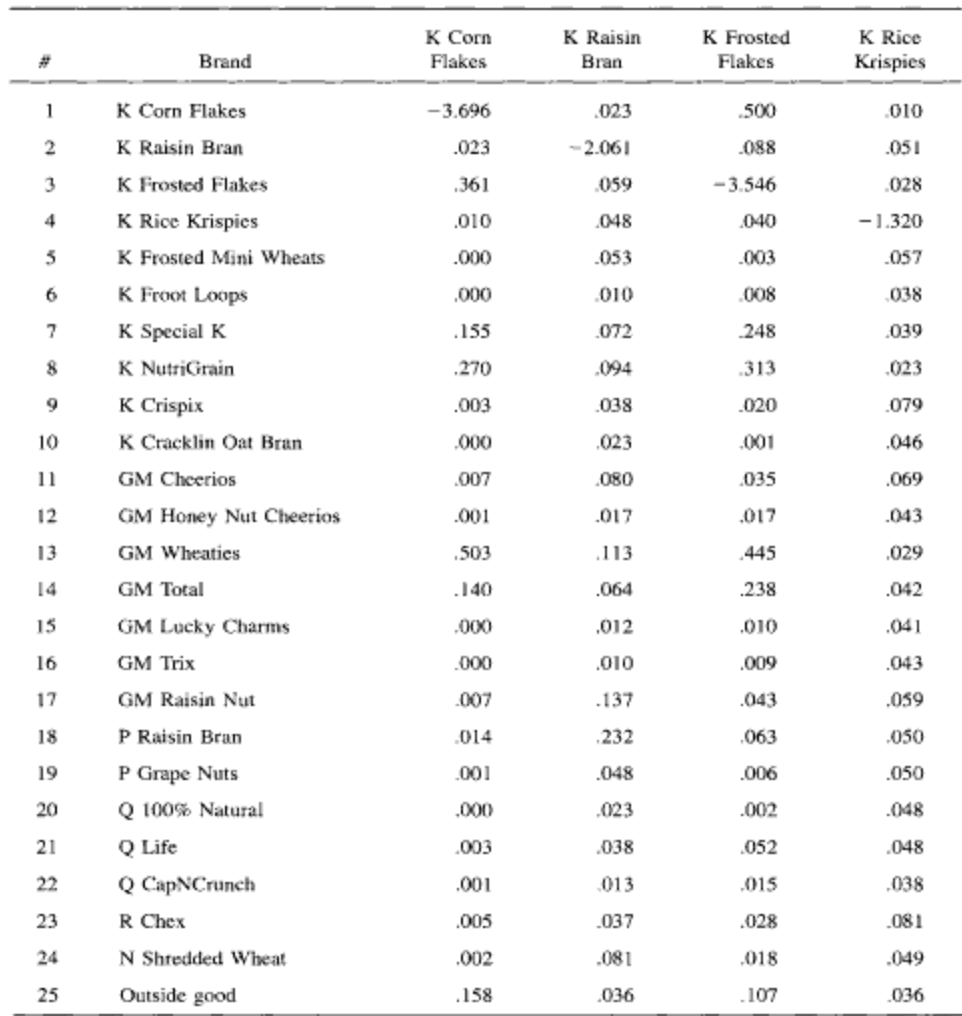
\includegraphics[height=\textheight]{./resources/nevo_elas.png}
\end{center}
\end{frame}


\begin{frame}{Advantages of Diversion}
\begin{itemize}
\item When you were taught elasticities you were taught they were a \alert{unit free} comparison across products, markets, etc.
\item But that is only true of \alert{own elasticities} not cross elasticities.
\item Is $\epsilon_{jt}=.01$ or $\epsilon_{jt}=.03$ a better substitute? We can't tell.
\begin{itemize}
\item You need to take $\epsilon_{jk} \cdot s_k$ to know. If you take $\epsilon_{jk} \cdot \frac{s_k}{p_j} = D_{jk}$ (back at diversion).
\item Because it tells us \alert{fraction of switchers} choosing $k$ we can compare across settings (since share sums to one).
\item ie: diversion ratio $D_{jk} = 0.1$ actually tells me something!
\end{itemize}
\item Whenever you are tempted to report \alert{cross elasticities} report \alert{diversion ratio} instead.
\end{itemize}
\end{frame}




%\begin{frame}
%\frametitle{Antitrust Policy -- Horizontal Mergers}
%Antitrust authorities use diversion ratios, a la Bertrand, to understand the `unilateral effects' of proposed mergers.
%\begin{itemize}
%\item Unilateral effects: competition between products of the merged firm is reduced because the merged firm internalizes substitution between jointly-owned products.
%\item Unilateral effects can lead to price increases.
%\item Current U.S. merger guidelines:\\
%\indent \textit{\footnotesize Diversion ratios between products [of the merging firms] can be very informative for assessing unilateral price effects.}
%\item Higher diversion between merging products pre-merger $\rightarrow$ greater scope for potential price increases.
%\end{itemize}
%\end{frame}

\section{Where do Diversion Ratios come from?\\ (Stolen from Conlon and Mortimer (2020)}
\begin{frame}{In Theory}
\footnotesize
Consider Bertrand FOC's for multi-product firm $j$:
\begin{align*}
\label{eq:best_response}
\rightarrow \nonumber p_j &=q_{j}(\mathbf{p}) \left[-\frac{\partial q_{j}}{\partial P_{j}}(\mathbf{p})\right]^{-1} + c_{j} + \sum_{k \in \mathcal{J}_{f} \setminus j} \left(p_{k}-c_{k}\right) \underbrace{\frac{\partial q_{k}}{\partial P_{j}}(\mathbf{p})\left[-\frac{\partial q_{j}}{\partial P_{j}}(\mathbf{p})\right]^{-1}}_{D_{jk}(\mathbf{p})}\\
p_j(p_{-j}) &= \underbrace{\frac{1}{1+1/\epsilon_{jj}(\mathbf{p})}}_{\text{Markup}} \left[ c_j + \sum_{k \in \mathcal{J}_{f} \setminus j}  (p_k-c_k) \cdot  D_{jk} (\mathbf{p}) \right].
\end{align*}
Mult-product pricing \alert{raises the opportunity cost} of selling $j$.
\end{frame}

\begin{frame}{Upward Pricing Pressure}
Agencies often calculate \alert{Upward Pricing Pressure} or UPP asks how merger \alert{changes}:
\begin{align*}
\left[ c_j + \sum_{k \in \mathcal{J}_{f} \setminus j}  (p_k-c_k) \cdot  D_{jk} (\mathbf{p}) \right] \\
UPP_j = \Delta c_j + \sum_{k \in \mathcal{J}_{g}}  (p_k-c_k) \cdot  D_{jk} (\mathbf{p}) 
\end{align*}
How does the merger change the \alert{opportunity cost} for $j$?
\end{frame}

\begin{frame}
\frametitle{UPP Extensions}
\begin{block}{Extension to multiple acquisitions:}
Very easy if we have that $p_j - mc_j = p - mc$ are the same for several values of $j$.  Then
\begin{eqnarray*}
UPP_j &\approx& (p - mc) \sum_k D_{jk}(\mathbf{p}) -  \Delta mc_j \\
\end{eqnarray*}
\end{block}
If several brands of acquisition have the same markup -- can consider firm-level diversion. (We can aggregate diversion across similar flavors)
\begin{block}{Ignoring Efficiencies}
\begin{eqnarray*}
GUPPI_j &\approx& \frac{(p_j - mc_j)}{p_j} D_{jk}(\mathbf{p}) \\
\end{eqnarray*}
\end{block}
\end{frame}


\begin{frame}
\frametitle{Diversion: In Practice}
\footnotesize
\begin{enumerate}
\item Calculated from an estimated demand system (ratio of estimated cross-price to own-price demand derivatives)
\item Consumer surveys (what would you buy if not this?)
\item Obtained in `course of business' (sales reps, internal reviews)
\end{enumerate}
Antitrust authorities may prefer different measures in different settings. Are they concerned about:
\begin{itemize}
\item Small but widespread price hikes?
\item Product discontinuations or changes to availability?
\end{itemize}
Is it sufficient to rely on data from merging firms only?
\begin{itemize}
\item Do we need diversion to other products in the `market' or other functions of market-level data?
\item Discrete-choice demand models imply that `aggregate diversion' (including to an outside good) sums to one.
\end{itemize}
\end{frame}


\begin{frame}{Wald Estimator}
The diversion ratio $D_{jk}(p_j,x) \equiv\frac{\partial q_k}{\partial P_j}(p_j,x)/-\frac{\partial q_j}{\partial P_j}(p_j,x)$ can be obtained as the limit of the Wald estimator where the price increase (or decrease) becomes small, so long as demand slopes \textit{strictly} downwards $\frac{\partial q_j}{\partial P_j} <0$.
\begin{align*}                               
\lim_{p_j' \rightarrow p_j} \frac{q_k(p_j',x) - q_k(p_j,x)}{-(q_j(p_j',x) - q_j(p_j,x))} \rightarrow \frac{\frac{\partial q_k}{\partial P_j}(p_j,x)}{-\frac{\partial q_j}{\partial P_j}(p_j,x)} \equiv D_{jk}(p_j,x)
\end{align*}
\end{frame}

\begin{frame}{Analogue to LATE Theorem Imbens Angrist (1994)}
\begin{theorem}[Conlon Mortimer (2020)]\ \\
\label{prop:late}
Under the following conditions:\\ 
(a) Mutually Exclusive and Exhaustive Discrete Choice: $d_{ij} \in \{0,1\}$ and $\sum_{j \in \mathcal{J}} d_{ij}=1$.\\
(b) Exclusion: $u_{ik}(p_j,x)=u_{ik}(p_j',x)$ for all $k \neq j$ and any $(p_j, p_j')$; \\
(c) Monotonicity: $u_{ij}(p_j',x) \leq u_{ij}(p_j,x)$ for all $i$ and any $(p_j' > p_{j})$; and \\
(d) Existence of a first-stage: $Pr(d_{ij}(p_j,x)=0) \neq Pr(d_{ij}(p_j',x)=0) $ for $(p_j' > p_{j})$; \\
(e) Random Assignment: $(u_{ij}(P_j,x),u_{ik}(P_j,x)) \perp P_j$. \\
\noindent
then the Wald estimator:
\begin{align*}
 \frac{q_k(p_j',x) - q_k(p_j,x)}{-\left(q_j(p_j',x) - q_j(p_j,x)\right)}=E[D_{jk,i}(x) | d_{ij}(p_j,x) > d_{ij}(p_j',x)]
\end{align*}
\end{theorem}
\end{frame}

\begin{frame}{Diversion as Treatment Effects}
\begin{description}
\item[Outcome] $Y_i \in \{0,1\}$ denotes the event that consumer $i$ purchases product $k$: $d_{ik}(P_j)=1$.
\item[Treatment] $T_i \in \{0,1\}$ denotes the event that consumer $i$ does \textbf{not} purchase product $j$. In other words $T_i = 0$ implies $d_{ij}(P_j)=1$ and $T_i=1$ implies $d_{ij}(P_j)=0$.
\item[Instrument] $Z_i = P_j$ the price of $j$ induces consumers into not purchasing $j$.
\end{description}
\end{frame}

\begin{frame}{Diversion as MTE}
\footnotesize
What can we learn from a change in $p_j$?
\begin{align*}
\text{Wald}(p_j, p_j',x)
&=\int_{p_j}^{p_j'} D_{jk}(p_s,x) w(p_s) \, \partial \, p_s \mbox{ with }
w(p_s)=\frac{  \frac{\partial q_j(p_s,x)}{\partial p_j} }{\int_{p_j}^{p_j'}  \frac{\partial q_j(p_t,x)}{\partial p_j} \partial p_t} \\
\nonumber &=\int_{p_j}^{p_j'} \int D_{jk,i}(p_s,x)  w_i(p_s,x) \, \partial p_s  \, \partial F_i \quad \mbox{ with } w_i(p_s,x) = \frac{\left| \frac{\partial q_{ij}(p_s,x)}{\partial p_j} \right|}{q_j(p_j,x)- q_j(p_j',x)}\\
&= \int D_{jk,i}(x) \, w_i(z_j,z_j',x)  \, \partial F_i \quad \mbox{ with } w_i(z_j,z_j',x) = \frac{q_{ij}(z_j,x)- q_{ij}(z_j',x) }{q_j(z_j,x)- q_j(z_j',x)}
\end{align*}
\begin{itemize}
\item Individual diversion ratios in logit family are $D_{jk,i} = \frac{s_{ik}}{1-s_{ij}}$ and don't depend on $p_j,z_j$
\item Which individuals respond to $z_j$ or $p_j$ determines the weighting scheme only.
\end{itemize}
\end{frame}

\begin{frame}{Weights}
Again $D_{jk,i} = \frac{s_{ik}}{1-s_{ij}}$ for logit family:\\
\begin{tabular}{rcc} 
& $w_{i j}(x) \propto$ \\
\midrule second choice data & $s_{i j}(x)$ \\
price change $\frac{\partial}{\partial p_{j}}$ & $s_{i j}(x) \cdot\left(1-s_{i j}(x)\right) \cdot\left|\alpha_{i}\right|$ \\
characteristic change $\frac{\partial}{\partial x_{j}}$ & $s_{i j}(x) \cdot\left(1-s_{i j}(x)\right) \cdot\left|\beta_{i}\right|$ \\
small quality change $\frac{\partial}{\partial \xi_{j}}$ & $s_{i j}(x) \cdot\left(1-s_{i j}(x)\right)$ \\
\midrule
\end{tabular}\\
For plain logit $D_{jk,i} = \frac{s_{k}}{1-s_{j}}$ for all $i$ and weights don't matter!
\end{frame}

\begin{frame}{Welfare and WTP}
As we learned on HW2, welfare and willingness to pay are mostly about \alert{diversion to outside good}
\begin{align*}
WTP_i(j) = E[\max_{k \in \mathcal{J}} u_{ik}]  - E[\max_{k' \in \mathcal{J}\setminus j} u_{ik'} ] =  \log \left( \sum_{k \in \mathcal{J}} \exp[V_{ik}] \right)-  \log \left(\sum_{k \in \mathcal{J} \setminus j} \exp[V_{ik}]\right)
\end{align*}
Exploit the following:
\begin{enumerate}
 \item the individual outside good choice probability $s_{i0}(\mathcal{J},x) = \frac{1}{ \sum_{k \in \mathcal{J}} \exp[V_{ik}]}$;
 \item  that the outside good choice probability after removing $j$ increases by the individual share of $j$ times the individual diversion ratio from $j$ to the outside good $s_{i0}(\mathcal{J}\setminus j,x)  = s_{i0}(\mathcal{J},x) + D_{j0,i}(x) \cdot s_{ij}(x)$; 
 \item for members of the logit family: $D_{j0,i}(x) = \frac{s_{i0}(x)}{1-s_{ij}(x)}$. 
\end{enumerate}
\end{frame}

\begin{frame}{Welfare and WTP}
To get EV we integrate over $\frac{1}{|\alpha_i|}$.
\begin{align*}
WTP_i(j) &=\log \left( \frac{s_{i0}(\mathcal{J}\setminus j,x) }{s_{i0}(\mathcal{J},x) }\right)
=\log \left( 1+\frac{D_{j0,i}(x) s_{ij}(x)}{s_{i0}(\mathcal{J},x) }\right)\\
&=\log \left( 1+\frac{s_{i0}(\mathcal{J},x) \cdot s_{ij}(x)}{(1-s_{ij}(x)) \cdot s_{i0}(\mathcal{J},x) }\right)\\
&=\log \left( 1+\frac{s_{ij}(x)}{1-s_{ij}(x)  }\right)
\approx \frac{s_{ij}(x)}{1-s_{ij}(x) }
\end{align*}
Individual willingness to pay is exclusively about \alert{own share} (not presence of close substitutes). Is this a good property or not?
\end{frame}


\begin{frame}{Practical Tips: Checklist}
\begin{itemize}
\item How much diversion to outside good?
\item What are top substitutes by diversion? How much do they get?
\item Do identities of best substitutes differ across products?
\item How much diversion goes to own products vs. competitors?
\item For mergers, what would \alert{divestiture} candidates be?
\end{itemize}
\end{frame}




\end{document}